% Provenance (never printed): see sources/outline_sources.md (Year 2: index minerals and zones,
% geothermometers and geobarometers, prograde and retrograde paths, metamorphic series,
% ultrahigh-pressure rocks and exhumation, ocean-floor metamorphism). Garnet-biotite
% calibration refitted from the Ferry and Spear (1978) brackets tabulated by Holdaway et al.
% (1997); GASP from Koziol and Newton (1988); thickening model after England and Thompson
% (1984) in figdata/bachelor-2/ptpaths.py; exercise and problem values in the Book 4 scratch
% calculators calc/ch11.py and calc/ch11b.py.
\chapter{Termobarometría y trayectorias P--T--t}\label{ch:b2:pt-paths}

Un granate de unos milímetros, crecido en un esquisto, conserva en su núcleo la composición
que tenía cuando empezó a crecer y en su borde la que tenía cuando dejó de hacerlo. Cada
zona estuvo en equilibrio con la biotita y la plagioclasa que la rodeaban en ese momento, y la
forma en que el hierro, el magnesio y el calcio se repartieron entre esos minerales depende de la temperatura
y de la presión. Leído con la termodinámica del capítulo anterior, un granate dice a qué
profundidad se enterró su roca y cuánto se calentó; datado, dice cuándo, y a qué velocidad
volvió a subir la roca. Este capítulo convierte los minerales metamórficos en termómetros, barómetros
y relojes, y sigue a una roca a lo largo de su trayectoria por la corteza.

\begin{recall}
\textbf{Del volumen de bachillerato}: el grado metamórfico, los minerales índice y las isogradas.
\textbf{Del volumen de primer año}: la geoterma y la producción de calor radiogénico; la
corteza continental de unos \qty{35}{km} de espesor; la datación radiométrica, la temperatura de cierre
de un mineral y la edad de enfriamiento que da; la corteza oceánica y su \omterm{def:b2:mantle-melting:peridotites}{peridotita}.
\textbf{De los libros de física}: la ecuación del calor $\partial T/\partial t = \kappa\,
\partial^2 T/\partial z^2$ y la difusividad térmica $\kappa$. \textbf{De los libros de
química}: la constante de equilibrio, $\Delta_r G^\circ + RT\ln K = 0$, y las actividades en
soluciones ideales. \textbf{Del \cref{ch:b2:metamorphic-facies}}: las reacciones metamórficas,
la \omterm{def:b2:metamorphic-facies:clapeyron}{pendiente de Clapeyron}, el diagrama \ce{Al2SiO5} y las facies.
\end{recall}
% ledger: prem:moho-average

\section{Las zonas metamórficas}\label{sec:b2:pt-paths:zones}

En las lutitas de las Highlands de Escocia, George Barrow cartografió en la década de 1890 una sucesión de
zonas, cada una marcada por la primera aparición de un nuevo mineral índice. Hacia el grado
más alto, a la clorita se le unen sucesivamente la biotita, el granate, la estaurolita, la cianita y la sillimanita;
en las secciones tipo las zonas del granate a la sillimanita se formaron a unos 500 a
\qty{650}{\celsius} y 5 a \qty{7}{kbar}.
% ledger: iugs:barrow, barrow1893:paper, earle:regional

\begin{definition}[Zonas barrovienses; gradiente metamórfico de campo]\label{def:b2:pt-paths:barrovian}
Las \emph{zonas barrovienses}\index{zonas barrovienses} son las zonas metamórficas de las
\omterm{def:b2:metamorphic-facies:protoliths}{metapelitas} en el orden clorita, biotita, granate, estaurolita, cianita, sillimanita,
cada una de las cuales empieza en la isograda de su mineral índice. El \emph{gradiente metamórfico de
campo}\index{gradiente metamórfico de campo} de una región es la curva, en el
plano presión--temperatura, que pasa por las condiciones de pico registradas por sus rocas en los
lugares donde afloran hoy.
\end{definition}

Cada punto de un gradiente de campo procede de una roca distinta, y cada roca alcanzó su propio
pico en su propio momento: el gradiente de campo no es la geoterma de ningún momento, ni la
trayectoria de ninguna roca. Es la traza que dejan los picos en la superficie de erosión actual.

\begin{omfigure}
\centering
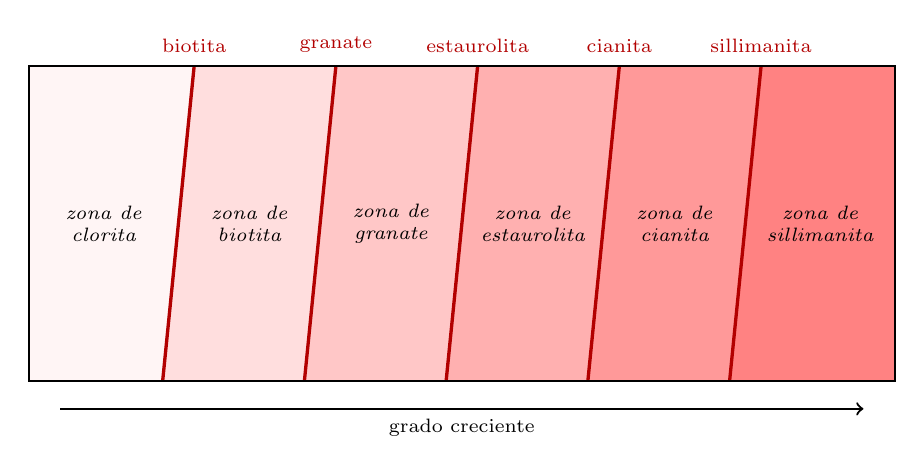
\begin{tikzpicture}[x=1cm, y=1cm]
\def\iso{{0,1.9,3.7,5.5,7.3,9.1,11}}
\foreach \i [evaluate=\i as \op using 4+9*\i] in {0,...,5} {
  \pgfmathsetmacro{\xa}{\iso[\i]}\pgfmathsetmacro{\xb}{\iso[\i+1]}
  \pgfmathsetmacro{\da}{(\i>0)*0.2}\pgfmathsetmacro{\db}{(\i<5)*0.2}
  \fill[red!\op!white] (\xa-\da,0) -- (\xb-\db,0) -- (\xb+\db,4) -- (\xa+\da,4) -- cycle;
}
\foreach \x/\n in {1.9/biotita, 3.7/granate, 5.5/estaurolita, 7.3/cianita, 9.1/sillimanita} {
  \draw[very thick, red!70!black] (\x-0.2,0) -- (\x+0.2,4);
  \node[font=\scriptsize, red!70!black, anchor=south] at (\x+0.2,4.05) {\n};
}
\draw[thick] (0,0) rectangle (11,4);
\foreach \x/\z in {0.95/clorita, 2.8/biotita, 4.6/granate, 6.4/estaurolita, 8.2/cianita, 10.05/sillimanita}
  \node[font=\scriptsize\itshape, align=center] at (\x,2) {zona de\\\z};
\draw[->, thick] (0.4,-0.35) -- node[below, font=\scriptsize] {grado creciente} (10.6,-0.35);
\end{tikzpicture}
\par\smallskip{\small \omterm{def:b2:pt-paths:barrovian}{Zonas barrovienses} en un mapa, esquema. Cada isograda (línea roja, con su nombre
encima del mapa) es la línea donde aparece por primera vez su mineral índice; el grado, y la intensidad
del sombreado, aumentan hacia la derecha. Cada zona lleva el nombre del mineral que aparece en su
límite de bajo grado.}
\end{omfigure}
% ledger: iugs:barrow

Las isogradas se cartografían a partir de apariciones de minerales, y solo se convierten en condiciones de presión y
temperatura cuando se conocen las reacciones que hay detrás. Para ir más lejos, hay que medir
la temperatura y la presión en una sola roca.

\section{Termómetros y barómetros}\label{sec:b2:pt-paths:thermobarometry}

\begin{definition}[Geotermómetro; geobarómetro; reacción de intercambio; reacción de transferencia neta]\label{def:b2:pt-paths:thermobarometry}
Un \emph{geotermómetro}\index{geotermómetro} (\emph{geobarómetro}\index{geobarómetro}) es
un equilibrio entre minerales cuya posición depende sobre todo de la temperatura (de la presión), de modo
que las composiciones de los minerales dan la temperatura (la presión) de su último
equilibrio. Una \emph{reacción de intercambio}\index{reacción de intercambio} intercambia dos elementos
entre dos minerales, como el hierro y el magnesio entre el granate y la biotita, sin
crear ni destruir ninguno de los dos minerales. Una \emph{reacción de transferencia neta}\index{reacción de transferencia neta}
forma unos minerales a expensas de otros.
\end{definition}

El termómetro más usado de las \omterm{def:b2:metamorphic-facies:protoliths}{metapelitas} es el intercambio de hierro y magnesio
entre el granate y la biotita,
\[
\ce{Fe3Al2Si3O12 + KMg3AlSi3O10(OH)2 <=> Mg3Al2Si3O12 + KFe3AlSi3O10(OH)2},
\]
almandino más flogopita que dan piropo más annita. Sean $X_{\text{Mg}}$ y $X_{\text{Fe}}$
las fracciones de los sitios ocupadas por el magnesio y el hierro en cada mineral, y
\[
K_D = \frac{(X_{\text{Mg}}/X_{\text{Fe}})_{\text{granate}}}{(X_{\text{Mg}}/X_{\text{Fe}})_{\text{biotita}}}.
\]
% ledger: h97:fs-reaction

\begin{proposition}[Un equilibrio de intercambio]\label{prop:b2:pt-paths:exchange}
Si el granate y la biotita son soluciones ideales y $\Delta_r H$, $\Delta_r S$ y $\Delta_r V$ de
la reacción anterior son constantes, entonces en el equilibrio
\[
3RT\ln K_D = -(\Delta_r H + P\,\Delta_r V) + T\,\Delta_r S,
\qquad\text{luego}\qquad
T = \frac{\Delta_r H + P\,\Delta_r V}{\Delta_r S - 3R\ln K_D}.
\]
\end{proposition}

\begin{proof}
Cada mineral tiene tres sitios para el hierro o el magnesio. En una solución ideal la actividad de
un miembro extremo es el producto de las fracciones de sus sitios que ocupa: $a_{\text{piropo}} =
X_{\text{Mg}}^3$ en el granate, y así sucesivamente. La constante de equilibrio es por tanto
\[
K = \frac{a_{\text{piropo}}\,a_{\text{annita}}}{a_{\text{almandino}}\,a_{\text{flogopita}}}
= \frac{X_{\text{Mg,grt}}^3\,X_{\text{Fe,bt}}^3}{X_{\text{Fe,grt}}^3\,X_{\text{Mg,bt}}^3} = K_D^3 .
\]
En el equilibrio $\Delta_r G^\circ(T, P) + RT\ln K = 0$, con $\Delta_r G^\circ = \Delta_r H -
T\,\Delta_r S + P\,\Delta_r V$ (despreciando el 1 de $P - 1$), lo que da la primera ecuación;
despejando $T$ se obtiene la segunda.
\end{proof}

Las constantes proceden de experimentos en los que granate y biotita sintéticos intercambiaron hierro
y magnesio a temperatura conocida y a \qty{2.07}{kbar}. Doce de esos intervalos, de 550 a
\qty{800}{\celsius}, representados como $\ln K_D$ frente a $1/T$, caen cerca de una recta (figura
siguiente); ajustados por mínimos cuadrados con $\Delta_r V = \qty{0.311}{J.bar^{-1}}$, dan
$\Delta_r H = \qty{52630}{J}$ y $\Delta_r S = \qty{20.19}{J.K^{-1}}$, los valores de los
recálculos publicados de los mismos datos. A mayor temperatura la razón $K_D$ sube
hacia 1: el granate toma una parte mayor del magnesio.
% ledger: h97:fs-data, h97:ideal, h97:fs-reaction

\begin{omfigure}
\centering
\begin{tikzpicture}
\begin{axis}[omrecord, width=0.62\linewidth, height=5.2cm,
  xmin=0.9, xmax=1.25, ymin=-1.9, ymax=-1.1,
  xlabel={$1000/T$ (\unit{K^{-1}})}, ylabel={$\ln K_D$},
  tick label style={font=\scriptsize}, label style={font=\small},
  x tick label style={/pgf/number format/.cd, fixed, precision=2}]
\addplot[only marks, mark=*, mark size=1.6pt, blue!70!black]
  table[x expr={1000/(\thisrow{T_C}+273.15)}, y=lnKD] {figdata/out/bachelor-2-ptpaths-fs.dat};
\addplot[thick, red!75!black, domain=0.9:1.25, samples=2] {(-52630-2070*0.311)/(3*8.31441)*x/1000 + 20.19/(3*8.31441)};
\end{axis}
\end{tikzpicture}
\par\smallskip{\small Intercambio granate--biotita: los doce intervalos experimentales a
\qty{2.07}{kbar} (azul, tal como los tabularon Holdaway y colaboradores, 1997) y la recta de
la proposición con los $\Delta_r H$ y $\Delta_r S$ ajustados (rojo).}
\end{omfigure}
% ledger: h97:fs-data, h97:ideal

Para $K_D = 0.18$ a \qty{5}{kbar}, $T = (52630 + 0.311\times5000)/(20.19 - 3\times8.314
\times\ln 0.18) = 54185/62.96 = \qty{861}{K}$, o sea \qty{587}{\celsius}. Un kilobar más
añade $0.311\times1000/62.96 = \qty{4.9}{K}$: la reacción intercambia iones de la misma carga
entre sitios de casi el mismo tamaño, su variación de volumen es pequeña, y la presión apenas
importa. Eso es lo que hace un termómetro.

Un barómetro necesita lo contrario: una reacción con una gran variación de volumen. La \omterm{def:b2:pt-paths:thermobarometry}{reacción
de transferencia neta}
\[
\ce{3 CaAl2Si2O8 <=> Ca3Al2Si3O12 + 2 Al2SiO5 + SiO2},
\]
anortita que da grosularia, cianita y cuarzo, empaqueta los átomos de tres feldespatos en
minerales más densos: $\Delta_r V = \qty{-6.21}{J.bar^{-1}}$, veinte veces la del intercambio.
Su equilibrio entre miembros extremos, invertido en experimentos de 900 a \qty{1250}{\celsius} y de 19
a \qty{28}{kbar}, sigue la recta
\[
P_0 = 22.80\,T - 1093 \qquad (P_0 \text{ en bar}, T \text{ en } \unit{\celsius}).
\]
En una roca, la grosularia es una pequeña parte del granate y la anortita una parte de la
plagioclasa. Con actividades ideales, $a_{\text{grosularia}} = X_{\text{Ca,grt}}^3$ y
$a_{\text{anortita}} = X_{\text{an}}$, la condición $\Delta_r G^\circ + RT\ln K = 0$
escrita a $P$ y a $P_0$ da
\[
P = P_0 + \frac{RT}{6.21}\,\ln\frac{X_{\text{Ca,grt}}^3}{X_{\text{an}}^3}
\qquad (T \text{ en kelvin en el segundo término}).
\]
Este \omterm{def:b2:pt-paths:thermobarometry}{geobarómetro}, llamado GASP por los cuatro minerales (granate, aluminosilicato, sílice,
plagioclasa), sirve allí donde una \omterm{def:b2:metamorphic-facies:protoliths}{metapelita} contiene los cuatro.
% ledger: kn88:gasp, rh95:gb-gasp

\begin{method}[Temperatura y presión de una roca]\label{met:b2:pt-paths:intersection}
(1) Mídanse, en minerales que crecieron juntos, las composiciones que necesitan el termómetro y el
barómetro. (2) Supóngase una presión y calcúlese la temperatura con el termómetro.
(3) A esa temperatura, calcúlese la presión con el barómetro. (4) Repítanse (2) y (3)
hasta que ninguna cambie; bastan dos o tres vueltas, ya que cada ecuación depende poco de
la variable que fija la otra. Gráficamente, la respuesta está donde la línea del
termómetro corta la del barómetro. (5) Propáguense las incertidumbres: para
errores independientes, $\sigma_T^2 = (\partial T/\partial\ln K_D)^2\sigma_{\ln K_D}^2 +
(\partial T/\partial P)^2\sigma_P^2$, y de forma análoga para $P$.
\end{method}

\begin{omfigure}
\centering
\begin{tikzpicture}
\begin{axis}[omrecord, width=0.78\linewidth, height=6.4cm,
  xmin=400, xmax=800, ymin=0, ymax=12, xlabel={$T$ (\unit{\celsius})}, ylabel={$P$ (\unit{kbar})},
  tick label style={font=\scriptsize}, label style={font=\small}, clip=false]
\addplot[thick, red!75!black] table[x=kd12, y=P_kbar] {figdata/out/bachelor-2-ptpaths-gb.dat};
\addplot[thick, red!75!black] table[x=kd15, y=P_kbar] {figdata/out/bachelor-2-ptpaths-gb.dat};
\addplot[thick, red!75!black] table[x=kd18, y=P_kbar] {figdata/out/bachelor-2-ptpaths-gb.dat};
\addplot[thick, red!75!black] table[x=kd21, y=P_kbar] {figdata/out/bachelor-2-ptpaths-gb.dat};
\addplot[thick, red!75!black] table[x=kd24, y=P_kbar] {figdata/out/bachelor-2-ptpaths-gb.dat};
\addplot[thick, blue!70!black] table[x=T_C, y=r15] {figdata/out/bachelor-2-ptpaths-gasp.dat};
\addplot[thick, blue!70!black] table[x=T_C, y=r20] {figdata/out/bachelor-2-ptpaths-gasp.dat};
\addplot[thick, blue!70!black] table[x=T_C, y=r25] {figdata/out/bachelor-2-ptpaths-gasp.dat};
\addplot[thick, blue!70!black] table[x=T_C, y=r30] {figdata/out/bachelor-2-ptpaths-gasp.dat};
\node[font=\tiny, red!75!black, anchor=west] at (axis cs:452,0.5) {0.12};
\node[font=\tiny, red!75!black, anchor=west] at (axis cs:511,0.5) {0.15};
\node[font=\tiny, red!75!black, anchor=west] at (axis cs:568,0.5) {0.18};
\node[font=\tiny, red!75!black, anchor=west] at (axis cs:622,0.5) {0.21};
\node[font=\tiny, red!75!black, anchor=west] at (axis cs:675,0.5) {0.24};
\node[font=\tiny, blue!70!black, anchor=west] at (axis cs:802,8.97) {0.15};
\node[font=\tiny, blue!70!black, anchor=west] at (axis cs:802,10.21) {0.20};
\node[font=\tiny, blue!70!black, anchor=west] at (axis cs:802,11.17) {0.25};
\node[font=\tiny, blue!70!black, anchor=west] at (axis cs:802,11.96) {0.30};
\end{axis}
\end{tikzpicture}
\par\smallskip{\small Isotermas granate--biotita (rojo, empinadas, rotuladas con $K_D$) e isobaras
GASP (azul, rotuladas a la derecha con la razón $X_{\text{Ca}}/X_{\text{an}}$ entre la
grosularia del granate y la anortita de la plagioclasa), según las calibraciones de esta sección. Una roca que contiene ambos pares está
donde se cortan sus dos líneas.}
\end{omfigure}
% ledger: h97:ideal, h97:fs-reaction, kn88:gasp

Las líneas del termómetro son casi verticales, las del barómetro inclinadas: se cortan con un
ángulo amplio, lo que mantiene precisa la intersección. La mezcla ideal es la principal simplificación
de este capítulo. Los granates reales contienen calcio y manganeso, las biotitas reales aluminio,
titanio y hierro férrico, y las calibraciones que los corrigen desplazan las temperaturas
decenas de grados (en una región bien estudiada, \qty{574}{\celsius} en lugar de
\qty{530}{\celsius}); las mejores declaran una incertidumbre de unos \qty{25}{\celsius}.
% ledger: h97:ideal, h97:corrections

\section{Trayectorias presión--temperatura}\label{sec:b2:pt-paths:paths}

Una roca no alcanza su presión máxima y su temperatura máxima en el mismo momento.
Se entierra y se calienta, después vuelve a subir y se enfría, y sus minerales reaccionan todo
el tiempo.

\begin{definition}[Trayectoria P--T; trayectorias prógrada y retrógrada; condiciones del pico metamórfico]\label{def:b2:pt-paths:paths}
La \emph{trayectoria P--T}\index{trayectoria P--T} de una roca es la sucesión de presiones y
temperaturas por las que pasó durante un episodio metamórfico. Su \emph{trayectoria
prógrada}\index{trayectoria prógrada} es la parte a lo largo de la cual sube la temperatura, su \emph{trayectoria
retrógrada}\index{trayectoria retrógrada} la parte a lo largo de la cual baja. Las \emph{condiciones del pico
metamórfico}\index{condiciones del pico metamórfico} son la presión y la temperatura en la
temperatura más alta de la trayectoria, el pico térmico; el pico de presión, o pico bárico, no tiene
por qué coincidir con él.
\end{definition}
% ledger: scmr:ptt

Una trayectoria es \emph{horaria} cuando, dibujada con la temperatura hacia la derecha y la presión hacia arriba,
el pico térmico llega después del pico bárico, durante la descompresión; es
\emph{antihoraria} cuando el pico térmico se alcanza mientras la presión aún sube. Qué
sentido sigue una roca depende de cómo le llegó el calor, y el caso más sencillo puede
calcularse.
% ledger: scmr:ptt

Imagínese una corteza de \qty{35}{km} de espesor, en estado estacionario, con una producción de calor de
\qty{1.0}{\micro W.m^{-3}}, un flujo de calor de \qty{25}{mW.m^{-2}} desde abajo, una conductividad
de \qty{2.5}{W.m^{-1}.K^{-1}} y una difusividad de \qty{1e-6}{m^2.s^{-1}}, estas tres últimas
dentro de los intervalos medidos en rocas. Su flujo de calor en superficie es de \qty{60}{mW.m^{-2}} y su Moho está a
\qty{595}{\celsius}. Una colisión apila una segunda copia de esta corteza encima de ella, deprisa
en comparación con el tiempo que necesita el calor para desplazarse: las rocas de la lámina inferior conservan sus
temperaturas pero quedan \qty{35}{km} más abajo, de modo que la geoterma se vuelve un diente de sierra, con
rocas a \qty{0}{\celsius} a \qty{35}{km} bajo rocas calientes de la lámina superior. La corteza tiene
ahora \qty{70}{km} de espesor y contiene el doble de roca productora de calor. Treinta millones de años después
del apilamiento, empieza la erosión, que retira \qty{35}{km} en 70 millones de años
(\qty{0.5}{mm.yr^{-1}}).
% ledger: delaney:conductivity, roy:granitic-k, vila:heat-production, prem:moho-average, et84:ptt

\begin{proposition}[Escala de tiempo de la relajación térmica]\label{prop:b2:pt-paths:relaxation}
En una capa de espesor $L$ cuyas dos caras se mantienen a temperatura fija, una perturbación
de temperatura de la forma $\sin(\pi z/L)$ decae como $e^{-t/\tau}$, con
\[
\tau = \frac{L^2}{\pi^2\kappa}.
\]
\end{proposition}

\begin{proof}
Escríbase $\theta(z, t) = f(t)\sin(\pi z/L)$, que se anula en $z = 0$ y en $z = L$. La ecuación
del calor $\partial\theta/\partial t = \kappa\,\partial^2\theta/\partial z^2$ da
$f'\sin(\pi z/L) = -\kappa(\pi/L)^2 f\sin(\pi z/L)$, luego $f' = -f/\tau$ con $\tau =
L^2/(\pi^2\kappa)$, y $f = f(0)\,e^{-t/\tau}$.
\end{proof}

El diente de sierra tiene una longitud de onda del orden del espesor de una lámina: con $L =
\qty{35}{km}$, $\tau = \qty{3.9}{Myr}$, y la cuña fría a \qty{35}{km} se borra en menos de
diez millones de años. Toda la corteza engrosada, $L = \qty{70}{km}$, se relaja en $\tau =
\qty{16}{Myr}$, de modo que el calentamiento continúa durante decenas de millones de años, hacia la geoterma mucho
más caliente que sostiene una corteza el doble de gruesa y con el doble de roca productora de calor.
La figura
siguiente muestra las geotermas calculadas.
% ledger: delaney:conductivity

\begin{omfigure}
\centering
\begin{tikzpicture}
\begin{axis}[omrecord, width=0.62\linewidth, height=6.6cm,
  xmin=0, xmax=1000, ymin=0, ymax=80, y dir=reverse,
  xlabel={$T$ (\unit{\celsius})}, ylabel={profundidad (\unit{km})},
  legend style={font=\scriptsize, at={(0.02,0.02)}, anchor=south west},
  tick label style={font=\scriptsize}, label style={font=\small}]
\addplot[thick, black] table[x=t0, y=z_km] {figdata/out/bachelor-2-ptpaths-geo.dat};
\addlegendentry{\qty{0}{Myr}}
\addplot[thick, blue!70!black] table[x=t10, y=z_km] {figdata/out/bachelor-2-ptpaths-geo.dat};
\addlegendentry{\qty{10}{Myr}}
\addplot[thick, orange!85!black] table[x=t30, y=z_km] {figdata/out/bachelor-2-ptpaths-geo.dat};
\addlegendentry{\qty{30}{Myr}}
\addplot[thick, red!75!black] table[x=t60, y=z_km] {figdata/out/bachelor-2-ptpaths-geo.dat};
\addlegendentry{\qty{60}{Myr}}
\end{axis}
\end{tikzpicture}
\par\smallskip{\small Geotermas tras duplicar por apilamiento una corteza de \qty{35}{km}, calculadas
con la ecuación del calor (profundidades bajo la superficie del momento; la erosión empieza a los
\qty{30}{Myr}). Negro: el diente de sierra justo después del apilamiento. La base de la corteza engrosada,
a \qty{595}{\celsius} al principio, supera los \qty{900}{\celsius} al cabo de 60 millones de años.}
\end{omfigure}
% ledger: et84:ptt

Sígase la roca que estaba en la superficie antes del apilamiento y queda a \qty{35}{km} justo
después de él, bajo \qty{9.6}{kbar}. En cinco millones de años se calienta de 0 a
\qty{395}{\celsius} sin moverse; al empezar la erosión ha alcanzado
\qty{558}{\celsius}. La erosión la hace subir entonces, pero el calor sigue llegando más deprisa de lo que
escapa: la roca aún se calienta cuando ha subido \qty{6}{km}, y alcanza su pico
térmico, \qty{593}{\celsius} a \qty{7.8}{kbar}, 43 millones de años después del apilamiento. Solo
entonces se enfría, pasando por \qty{405}{\celsius} a \qty{13}{km} de profundidad y
\qty{74}{Myr}, camino de la superficie. La trayectoria (figura siguiente) es horaria. Además
permanece a menos de \qty{50}{\celsius} de su temperatura de pico durante treinta millones de años, cerca de un
tercio de todo su recorrido, como hallaron England y Thompson en 1984 para la mayoría de los casos
geológicamente plausibles: una roca pasa mucho tiempo cerca de su pico, y los minerales que conserva
registran sobre todo esa etapa.
% ledger: et84:ptt

\begin{omfigure}
\centering
\begin{tikzpicture}
\begin{axis}[omrecord, width=0.78\linewidth, height=6.2cm,
  xmin=0, xmax=800, ymin=0, ymax=11, xlabel={$T$ (\unit{\celsius})}, ylabel={$P$ (\unit{kbar})},
  tick label style={font=\scriptsize}, label style={font=\small}]
\addplot[thick, gray, densely dashed, restrict x to domain=0:504] table[x=T_C, y=P_kbar] {figdata/out/bachelor-2-facies-hm93-kyand.dat};
\addplot[thick, gray, densely dashed] table[x=T_C, y=P_kbar] {figdata/out/bachelor-2-facies-hm93-kysil.dat};
\addplot[thick, gray, densely dashed] table[x=T_C, y=P_kbar] {figdata/out/bachelor-2-facies-hm93-andsil.dat};
\addplot[very thick, red!75!black, postaction={decorate}, decoration={markings,
  mark=at position 0.2 with {\arrow{Stealth[length=2.5mm]}},
  mark=at position 0.52 with {\arrow{Stealth[length=2.5mm]}},
  mark=at position 0.8 with {\arrow{Stealth[length=2.5mm]}}}] table[x=T_C, y=P_kbar] {figdata/out/bachelor-2-ptpaths-path.dat};
\node[font=\scriptsize\bfseries, gray] at (axis cs:330,6.5) {cianita};
\node[font=\scriptsize\bfseries, gray] at (axis cs:520,1.0) {andalucita};
\node[font=\scriptsize\bfseries, gray] at (axis cs:740,4.0) {sillimanita};
\node[font=\scriptsize, red!75!black, anchor=south] at (axis cs:200,9.7) {calentamiento en profundidad};
\node[font=\scriptsize, red!75!black, anchor=west] at (axis cs:603,8.9) {pico térmico};
\node[font=\scriptsize, red!75!black, anchor=west] at (axis cs:110,2.7) {ascenso con enfriamiento};
\end{axis}
\end{tikzpicture}
\par\smallskip{\small \omterm{def:b2:pt-paths:paths}{Trayectoria P--T} de la roca que queda a \qty{35}{km} justo después del
apilamiento (rojo, muestreada cada dos millones de años), calculada con el modelo de las geotermas anteriores,
sobre el diagrama \ce{Al2SiO5} experimental del \cref{ch:b2:metamorphic-facies} (gris). El
pico de presión llega primero, el pico térmico durante la descompresión: una trayectoria horaria, que
nunca sale del campo de la cianita.}
\end{omfigure}
% ledger: et84:ptt, hm93:table11

El modelo muestra también por qué algunas trayectorias giran en sentido contrario. El engrosamiento por sí solo calienta una roca
solo después de que se haya enterrado, de modo que su pico térmico llega durante la \omterm{def:b2:pt-paths:exhumation}{exhumación}. Una roca cuya
temperatura sube mientras aún se está enterrando necesita calor de otra procedencia, como un \omterm{def:b2:magma-emplacement:magma}{magma}
que asciende en la corteza por encima o al lado de ella, y sigue una trayectoria antihoraria. Y en la
corteza engrosada la base se calienta muy por encima de su temperatura inicial: England y Thompson
concluyeron que una fusión considerable de la corteza es una consecuencia probable del engrosamiento,
el tema del \cref{ch:b2:crustal-melting}.
% ledger: et84:ptt, scmr:ptt

\section{Añadir el tiempo}\label{sec:b2:pt-paths:time}

\begin{definition}[Trayectoria P--T--t]\label{def:b2:pt-paths:ptt}
La \emph{trayectoria P--T--t}\index{trayectoria P--T--t} de una roca es su \omterm{def:b2:pt-paths:paths}{trayectoria P--T} con el momento en
que se alcanzó cada punto.
\end{definition}
% ledger: scmr:ptt

El tiempo procede de la datación radiométrica. Un mineral que creció durante el episodio y ha conservado
desde entonces sus isótopos hijos, como una zona de granate datada por el
método samario--neodimio, data su propio crecimiento, y su
composición da la presión y la temperatura de ese momento. Un mineral que creció
antes, a mayor temperatura, da en cambio una edad de enfriamiento: el momento en que la roca
se enfrió por debajo de la temperatura de cierre de ese mineral y ese sistema isotópico (volumen de primer
año). Para el argón en un grano de moscovita de \qty{100}{\micro m} de radio, que se enfría a
\qty{10}{\celsius} por millón de años, la temperatura de cierre es de \qty{405}{\celsius} a
\qty{5}{kbar} y de \qty{425}{\celsius} a \qty{10}{kbar}.
% ledger: h09:muscovite

\begin{definition}[Exhumación; tasa de exhumación]\label{def:b2:pt-paths:exhumation}
La \emph{exhumación}\index{exhumación} es el desplazamiento de una roca hacia la superficie de la Tierra,
por retirada de las rocas que tiene encima. La \emph{tasa de exhumación}\index{tasa de exhumación} es la
velocidad a la que disminuye su profundidad.
\end{definition}

\begin{proposition}[Velocidades a partir de dos puntos datados]\label{prop:b2:pt-paths:rates}
Si una roca estaba a la temperatura $T_1$ y a la profundidad $z_1$ en el momento $t_1$ y a $T_2$, $z_2$ en un
momento posterior $t_2$ (edades contadas hacia atrás desde hoy, $t_1 > t_2$), sus velocidades medias de enfriamiento y
de \omterm{def:b2:pt-paths:exhumation}{exhumación} en el intervalo son
\[
\frac{T_1 - T_2}{t_1 - t_2}
\qquad\text{y}\qquad
\frac{z_1 - z_2}{t_1 - t_2},
\]
y sus incertidumbres, para errores independientes en las dos edades, se deducen de
$\sigma_{t_1 - t_2}^2 = \sigma_{t_1}^2 + \sigma_{t_2}^2$.
\end{proposition}

\begin{proof}
Una velocidad media es una diferencia dividida por el tiempo transcurrido $t_1 - t_2$; la varianza de una
diferencia de magnitudes independientes es la suma de sus varianzas.
\end{proof}

La profundidad a la que se fijó una edad de enfriamiento rara vez se mide: se estima a partir de la
geoterma de la época, y por eso las \omterm{def:b2:pt-paths:exhumation}{tasas de exhumación} son menos seguras que las velocidades de enfriamiento.
Una presión, cuando una \omterm{def:b2:metamorphic-facies:assemblage}{asociación mineral} la proporciona, fija directamente la profundidad, como
$z = P/(\bar\rho g)$ con $\bar\rho$ la densidad media de las rocas suprayacentes.

\section{Series metamórficas y cinturones pareados}\label{sec:b2:pt-paths:series}

\begin{definition}[Serie metamórfica; cinturones metamórficos pareados]\label{def:b2:pt-paths:series}
Una \emph{serie metamórfica}\index{serie metamórfica} (o serie de facies) es una sucesión de
\omterm{def:b2:metamorphic-facies:facies}{facies metamórficas} desarrolladas en un mismo intervalo de razones entre presión y temperatura,
y que ocupan por tanto un sector radial del plano presión--temperatura.
Los \emph{cinturones metamórficos pareados}\index{cinturones metamórficos pareados} son dos cinturones paralelos de
la misma edad, uno de series de alta presión y otro de series de baja presión.
\end{definition}
% ledger: scmr:ptt, wallis24:paired

Se suelen distinguir tres series. Una razón alta entre presión y temperatura, a lo largo de un
gradiente frío, lleva de la facies de las zeolitas a los esquistos azules y las eclogitas: la serie
de las zonas de subducción. Una razón intermedia pasa por las facies de los esquistos verdes, las anfibolitas y las
granulitas, con cianita y después sillimanita en las \omterm{def:b2:metamorphic-facies:protoliths}{metapelitas}: la serie barroviense. Una razón
baja, a lo largo de gradientes calientes como los que hay cerca de las intrusiones, produce andalucita y después
sillimanita: la serie de baja presión o de Buchan. La figura siguiente dibuja tres gradientes
a través del diagrama de los aluminosilicatos.
% ledger: scmr:ptt, scmr:facies, iugs:barrow, fub:paired

\begin{omfigure}
\centering
\begin{tikzpicture}
\begin{axis}[omrecord, width=0.78\linewidth, height=6.2cm,
  xmin=0, xmax=900, ymin=0, ymax=12, xlabel={$T$ (\unit{\celsius})}, ylabel={$P$ (\unit{kbar})},
  tick label style={font=\scriptsize}, label style={font=\small}]
\addplot[thick, gray, densely dashed, restrict x to domain=0:504] table[x=T_C, y=P_kbar] {figdata/out/bachelor-2-facies-hm93-kyand.dat};
\addplot[thick, gray, densely dashed] table[x=T_C, y=P_kbar] {figdata/out/bachelor-2-facies-hm93-kysil.dat};
\addplot[thick, gray, densely dashed] table[x=T_C, y=P_kbar] {figdata/out/bachelor-2-facies-hm93-andsil.dat};
\addplot[very thick, blue!70!black] table[x=T_C, y=g10] {figdata/out/bachelor-2-ptpaths-series.dat};
\addplot[very thick, green!45!black] table[x=T_C, y=g25] {figdata/out/bachelor-2-ptpaths-series.dat};
\addplot[very thick, orange!85!black] table[x=T_C, y=g60] {figdata/out/bachelor-2-ptpaths-series.dat};
\node[font=\scriptsize, blue!70!black, rotate=52, anchor=south] at (axis cs:330,8.5) {\qty{10}{\celsius\per\km}};
\node[font=\scriptsize, green!45!black, rotate=28, anchor=south] at (axis cs:640,7.0) {\qty{25}{\celsius\per\km}};
\node[font=\scriptsize, orange!85!black, rotate=12, anchor=south] at (axis cs:800,3.65) {\qty{60}{\celsius\per\km}};
\node[font=\scriptsize\bfseries, gray] at (axis cs:120,5.5) {cianita};
\node[font=\scriptsize\bfseries, gray] at (axis cs:470,1.1) {andalucita};
\node[font=\scriptsize\bfseries, gray] at (axis cs:800,1.6) {sillimanita};
\end{axis}
\end{tikzpicture}
\par\smallskip{\small Tres gradientes geotérmicos desde una superficie a \qty{10}{\celsius},
convertidos en presión con una densidad media de \qty{2800}{kg.m^{-3}}, sobre el diagrama
\ce{Al2SiO5} experimental (gris). El gradiente frío se queda en el campo de la cianita, el
intermedio pasa de la cianita a la sillimanita, y el caliente atraviesa el campo de la andalucita
antes de alcanzar la sillimanita.}
\end{omfigure}
% ledger: hm93:table11

La idea de las series vino de Japón, donde Akiho Miyashiro las definió en 1961. En
el suroeste del país el cinturón de Sanbagawa, de \omterm{def:b2:metamorphic-facies:metamorphism}{metamorfismo} de alta presión y baja temperatura,
se extiende más de \qty{800}{km} junto al cinturón de Ryoke, de \omterm{def:b2:metamorphic-facies:metamorphism}{metamorfismo} de alta temperatura y
baja presión, separados ambos por una falla mayor: el par clásico. El
cinturón de Sanbagawa es una antigua zona de subducción, el de Ryoke el arco volcánico que había encima. Una
zona de subducción produce así ambas series a la vez, rocas frías arrastradas hacia abajo por la placa
que se hunde, rocas calientes calentadas en el arco; se conocen cinturones pareados del mismo tipo alrededor del
Pacífico.
% ledger: wallis24:paired, koguchi17:paired, fub:paired, scmr:ptt

\section{Ultra alta presión y exhumación}\label{sec:b2:pt-paths:uhp}

En 1984 se describió en el macizo de Dora Maira, en los Alpes occidentales, una cuarcita
cuyos granates, de hasta \qty{25}{cm} y de piropo casi puro, encierran granos de
coesita, el polimorfo denso de la sílice, en parte retransformada en cuarzo; la expansión
durante esa inversión agrietó radialmente el granate huésped alrededor de cada grano. La coesita y
sus acompañantes implican al menos \qty{28}{kbar} a unos \qty{700}{\celsius}: rocas de la
corteza continental superior, antiguos sedimentos, habían descendido a \qty{90}{km} o más y habían
vuelto.
% ledger: chopin84:coesite

\begin{definition}[Metamorfismo de ultra alta presión]\label{def:b2:pt-paths:uhp}
El \emph{metamorfismo de ultra alta presión}\index{metamorfismo de ultra alta presión} es el
\omterm{def:b2:metamorphic-facies:metamorphism}{metamorfismo} de rocas corticales a presiones lo bastante altas para que crezca coesita, o diamante.
\end{definition}

\begin{omfigure}
\centering
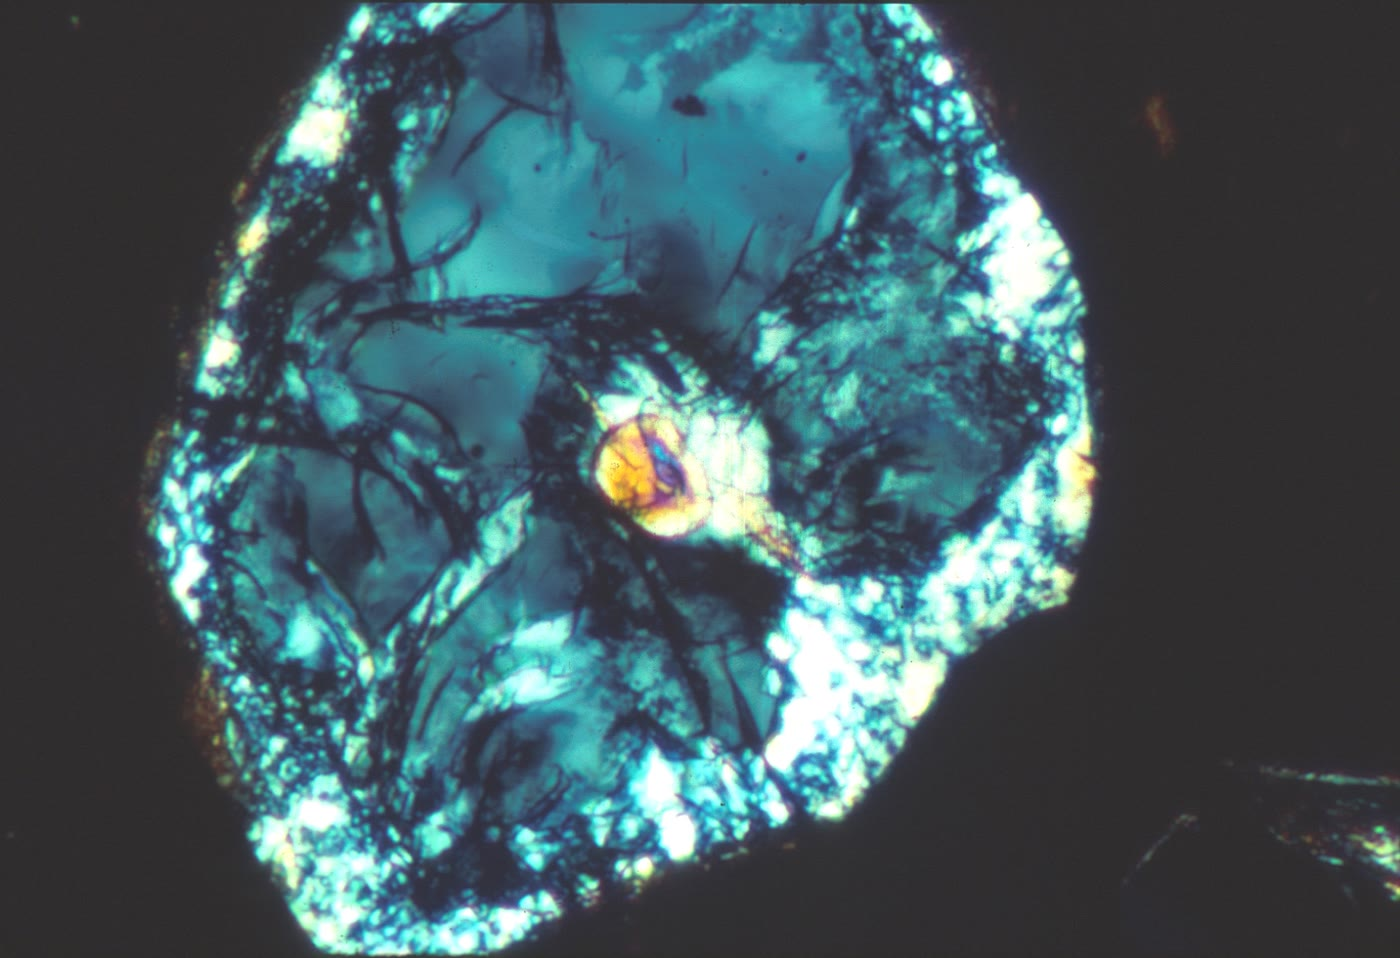
\includegraphics[width=0.62\linewidth]{images/book4/b2-11-coesite.jpg}
\par\smallskip{\small Coesita en una eclogita, de cerca de \qty{1}{mm}, en lámina delgada
con polarizadores cruzados: el gran grano central es coesita, el borde de pequeños granos brillantes es
cuarzo que creció a partir de ella al bajar la presión; el pequeño grano coloreado del centro es una
inclusión de piroxeno. Fotografía de J.\,R. Smyth, CC BY-SA 1.0.}
\end{omfigure}

Seis años después, se hallaron diamantes de \qty{12}{\micro m} de media en gneises, esquistos y
rocas de granate y piroxeno del macizo de Kokchetav, en el norte de Kazajistán, encerrados en granate
y circón, que los protegieron de transformarse en grafito: crecieron a \qty{40}{kbar}
o más y por encima de 900 a \qty{1000}{\celsius}. La corteza continental, aun siendo ligera, puede
ser arrastrada a más de cien kilómetros de profundidad.
% ledger: ss90:diamond

Cómo vuelve lo cuentan sus relojes. En las rocas subducidas más profundas de los Alpes,
la titanita datada en etapas sucesivas muestra que una roca calcosilicatada alcanzó unos
\qty{3.5}{GPa} a $35.1 \pm \qty{0.9}{Ma}$, estaba a $1 \pm \qty{0.15}{GPa}$ a $32.9 \pm
\qty{0.9}{Ma}$, y cerca de 0.4 a \qty{0.5}{GPa} a $31.8 \pm \qty{0.5}{Ma}$. Las tasas medias
de \omterm{def:b2:pt-paths:exhumation}{exhumación}, 3.4 y después \qty{1.6}{cm.yr^{-1}}, igualan las velocidades de las placas: las rocas
volvieron más o menos tan deprisa como bajaron, mucho más deprisa de lo que la erosión habría podido
desenterrarlas. Los autores invocan la flotabilidad, la corteza ligera que sube a través del manto más denso, y
las fallas normales, que adelgazan las rocas suprayacentes.
% ledger: rh01:exhumation

\section{El metamorfismo de fondo oceánico}\label{sec:b2:pt-paths:ocean-floor}

\begin{definition}[Metamorfismo de fondo oceánico; serpentinización]\label{def:b2:pt-paths:ocean-floor}
El \emph{metamorfismo de fondo oceánico}\index{metamorfismo de fondo oceánico} es el \omterm{def:b2:metamorphic-facies:metamorphism}{metamorfismo}
regional de la litosfera oceánica cerca de los centros de expansión, por fluidos acuosos calientes
que circulan con fuertes gradientes geotérmicos; la recristalización suele ser incompleta
y la temperatura suele aumentar con la profundidad. La \emph{serpentinización}\index{serpentinización}
es la hidratación de rocas ricas en olivino que las transforma en serpentina.
\end{definition}
% ledger: scmr:types

El agua de mar que penetra en la corteza joven cerca del eje de una dorsal se calienta, reacciona con las rocas y
vuelve a subir. Los basaltos que atraviesa recristalizan, de forma incompleta, en minerales
hidratados, en un amplio intervalo de temperaturas. Donde el agua alcanza la \omterm{def:b2:mantle-melting:peridotites}{peridotita}, como en
las dorsales lentas donde la roca del manto llega al fondo marino y alimenta fuentes como
las del campo hidrotermal de Lost City (volumen de primer año), el olivino incorpora agua:
\[
\ce{2 Mg2SiO4 + 3 H2O -> Mg3Si2O5(OH)4 + Mg(OH)2},
\]
la forsterita da serpentina y brucita. Los volúmenes molares, 43.65 para la forsterita, 107.50
para la serpentina y \qty{24.63}{cm^3.mol^{-1}} para la brucita, muestran lo que esto hace a la roca:
\qty{87.30}{cm^3} de olivino se convierten en \qty{132.13}{cm^3} de sólidos, un \qty{51}{\percent}
más, y la densidad baja de 3.22 a \qty{2.54}{g.cm^{-3}}. La roca se hincha y
se aligera, y el agua que ha fijado desciende con ella cuando la placa subduce.
% ledger: scmr:types, rh95:serpentine, kelley:lost-city, dick:ultraslow

\begin{inthelab}[Leer un granate]
Para leer una \omterm{def:b2:pt-paths:paths}{trayectoria P--T}, el petrólogo corta primero una lámina delgada por el centro de un
granate, ya que una sección descentrada no pasa por el núcleo. Al microscopio se cartografían las inclusiones:
pequeños granos de cuarzo, biotita, plagioclasa o cianita atrapados mientras el granate
crecía, a veces alineados en trenes que conservan una foliación más antigua de la roca. Una microsonda
electrónica mide después la composición a lo largo de una línea del núcleo al borde, y un mapa de
magnesio, hierro, calcio y manganeso muestra las zonas de crecimiento. Cada zona se empareja con
los minerales que crecieron con ella: las inclusiones para el núcleo, la matriz en contacto para el
borde. El termómetro y el barómetro se aplican a cada par, y las zonas se datan cuando un
mineral lo permite. El \cref{ch:b2:field-lab-methods-2} describe los instrumentos.
\end{inthelab}

\begin{omfigure}
\centering
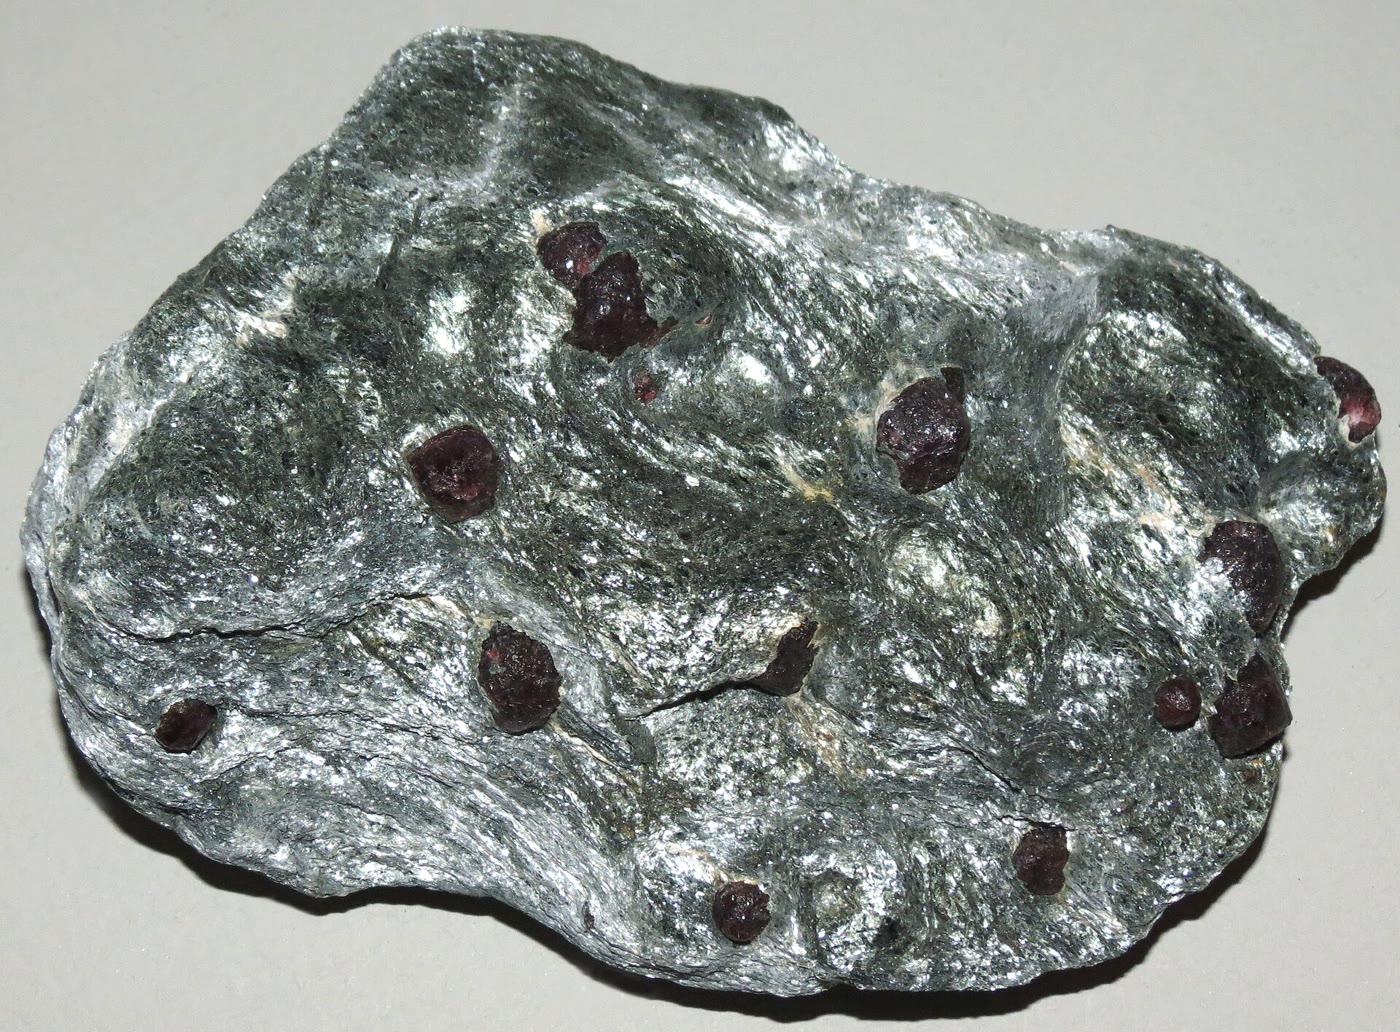
\includegraphics[width=0.62\linewidth]{images/book4/b2-11-garnet-schist.jpg}
\par\smallskip{\small Un esquisto con granate: cristales de granate rojo oscuro crecidos en una
matriz foliada de micas. Cada granate puede conservar, del núcleo al borde, un
registro de la trayectoria de la roca. Fotografía de James St.~John, CC BY 2.0.}
\end{omfigure}

\section{Ejercicios}

\begin{exercise}[$\star$]\label{exo:b2:pt-paths:1}
Seis muestras de una misma formación de lutitas, recogidas a lo largo de una carretera, contienen: (A) clorita,
moscovita, cuarzo; (B) biotita, clorita, moscovita, cuarzo; (C) granate, biotita,
moscovita, cuarzo; (D) estaurolita, granate, biotita, moscovita, cuarzo; (E) cianita,
estaurolita, biotita, moscovita, cuarzo; (F) sillimanita, biotita, moscovita, cuarzo.
(a) ¿En qué zona barroviense está cada una? (b) ¿Cuántas isogradas cruza la carretera, y
cuáles? (c) ¿Por qué no basta con conocer las isogradas para trazar el \omterm{def:b2:pt-paths:barrovian}{gradiente metamórfico
de campo}?
\end{exercise}
% ledger: iugs:barrow

\begin{exercise}[$\star$]\label{exo:b2:pt-paths:2}
Un granate tiene $X_{\text{Mg}} = 0.10$ y $X_{\text{Fe}} = 0.80$, la biotita que hay a su lado
$X_{\text{Mg}} = 0.45$ y $X_{\text{Fe}} = 0.50$. (a) Calcúlense $K_D$ y $\ln K_D$.
(b) Con la calibración de este capítulo, calcúlese la temperatura a \qty{5}{kbar} y a
\qty{7}{kbar}. (c) ¿Es el resultado un indicador de temperatura o de presión?
\end{exercise}
% ledger: h97:ideal, h97:fs-reaction

\begin{exercise}[$\star$]\label{exo:b2:pt-paths:3}
Una \omterm{def:b2:metamorphic-facies:protoliths}{metapelita} da \qty{580}{\celsius} y \qty{6.0}{kbar}. (a) Bajo rocas de densidad media
\qty{2800}{kg.m^{-3}} ($g = \qty{9.81}{m.s^{-2}}$), ¿a qué profundidad estaba? (b) ¿Qué
gradiente de temperatura implica desde \qty{10}{\celsius} en la superficie? (c) La
línea experimental cianita $=$ sillimanita pasa por \qty{3.67}{kbar} a
\qty{500}{\celsius} y por \qty{5.77}{kbar} a \qty{600}{\celsius}: ¿qué aluminosilicato
debería contener la roca?
\end{exercise}
% ledger: hm93:table11

\begin{exercise}[$\star$]\label{exo:b2:pt-paths:4}
Para la \omterm{def:b2:pt-paths:ocean-floor}{serpentinización} de la forsterita escrita en este capítulo: (a) compruébese que la
ecuación está ajustada en masa, con las masas molares 140.693 (forsterita), 18.015 (agua),
277.112 (serpentina) y \qty{58.320}{g.mol^{-1}} (brucita); (b) calcúlese la variación de
volumen de los sólidos; (c) calcúlense las densidades del olivino y de los productos.
(d) ¿Qué efecto tiene el cambio en una \omterm{def:b2:mantle-melting:peridotites}{peridotita} serpentinizada bajo el fondo marino?
\end{exercise}
% ledger: rh95:serpentine

\begin{exercise}[$\star\star$]\label{exo:b2:pt-paths:5}
Calíbrese el termómetro a partir de cuatro de los experimentos a \qty{2.07}{kbar}: $\ln K_D =
-1.157$ y $-1.255$ a \qty{799}{\celsius}, $-1.738$ y $-1.826$ a \qty{550}{\celsius}.
(a) Promédiese cada par y hállese la recta $\ln K_D = a/T + b$ que pasa por las dos medias.
(b) Dedúzcanse $\Delta_r H$ y $\Delta_r S$, con $\Delta_r V = \qty{0.311}{J.bar^{-1}}$.
(c) Compárense las temperaturas que dan su calibración y la del capítulo a
\qty{5}{kbar} para $K_D = 0.18$, $0.10$ y $0.30$. ¿Qué se concluye sobre la
extrapolación de una calibración?
\end{exercise}
% ledger: h97:fs-data, h97:ideal

\begin{exercise}[$\star\star$]\label{exo:b2:pt-paths:6}
(a) A partir de los volúmenes molares a \qty{298}{K} (almandino 115.32, piropo 113.12, annita
154.30, flogopita 149.65, grosularia 125.28, anortita 100.79, cianita 44.15, cuarzo
\qty{22.69}{cm^3.mol^{-1}}), calcúlese el $\Delta_r V$ del intercambio y de la reacción
GASP, y compárese con los valores que usan las calibraciones, \num{0.311} y
\qty{-6.21}{J.bar^{-1}}. (b) Para $K_D = 0.18$, ¿cuántos kelvin desplaza la temperatura un error de
\qty{1}{kbar}? (c) A lo largo de la línea GASP de una roca con
$X_{\text{Ca}}/X_{\text{an}} = 0.20$, ¿cuántos bares desplaza la presión
un error de \qty{17}{K}?
\end{exercise}
% ledger: rh95:gb-gasp, rh95:al2sio5, h97:fs-reaction, kn88:gasp

\begin{exercise}[$\star\star$]\label{exo:b2:pt-paths:7}
A \qty{600}{\celsius}, un granate tiene $X_{\text{Ca}} = 0.08$ y la plagioclasa que hay a su lado
$X_{\text{an}} = 0.30$. (a) Calcúlese la presión GASP. (b) Rehágase con $X_{\text{an}} =
0.35$. (c) ¿A qué profundidad estaba la roca, para una densidad media de \qty{2800}{kg.m^{-3}}?
\end{exercise}
% ledger: kn88:gasp

\begin{exercise}[$\star\star$]\label{exo:b2:pt-paths:8}
Úsense las edades de titanita de las rocas subducidas más profundas de los Alpes: unos \qty{3.5}{GPa} a
$35.1 \pm \qty{0.9}{Ma}$, \qty{1.0}{GPa} a $32.9 \pm \qty{0.9}{Ma}$, \qty{0.45}{GPa} a
$31.8 \pm \qty{0.5}{Ma}$. (a) Con una densidad media de \qty{3000}{kg.m^{-3}}, conviértanse las
presiones en profundidades. (b) Calcúlense las dos tasas medias de \omterm{def:b2:pt-paths:exhumation}{exhumación} y compárense con los
valores publicados, 3.4 y \qty{1.6}{cm.yr^{-1}}. (c) ¿Cuál es la incertidumbre del primer intervalo
de tiempo, y qué intervalo de velocidades permite? (d) Compárese con la velocidad de erosión
del modelo de engrosamiento, \qty{0.5}{mm.yr^{-1}}.
\end{exercise}
% ledger: rh01:exhumation

\begin{exercise}[$\star\star$]\label{exo:b2:pt-paths:9}
Para $K_D = 0.18$ a \qty{5}{kbar}, (a) calcúlense $\partial T/\partial\ln K_D$ y
$\partial T/\partial P$ a partir de la proposición; (b) con $\sigma_{\ln K_D} = 0.05$ (un
error del \qty{5}{\percent} en $K_D$) y $\sigma_P = \qty{1}{kbar}$, calcúlese $\sigma_T$.
(c) ¿Qué error domina? Compárese con la incertidumbre de \qty{25}{\celsius} que se atribuye a
las mejores calibraciones.
\end{exercise}
% ledger: h97:ideal

\begin{exercise}[$\star\star\star$]\label{exo:b2:pt-paths:10}
El borde de un granate tiene $X_{\text{Mg}} = 0.10$, $X_{\text{Fe}} = 0.75$, $X_{\text{Ca}} = 0.07$;
la biotita de la matriz $X_{\text{Mg}} = 0.42$, $X_{\text{Fe}} = 0.52$; la plagioclasa
$X_{\text{an}} = 0.25$. (a) Aplíquese el método de este capítulo, partiendo de \qty{6}{kbar},
hasta que la temperatura cambie menos de \qty{1}{K}. (b) ¿Qué aluminosilicato debería contener
la roca (úsese la línea experimental del \cref{exo:b2:pt-paths:3})? (c) ¿Por qué debe usar el barómetro
el aluminosilicato realmente presente?
\end{exercise}
% ledger: h97:ideal, kn88:gasp, hm93:table11

\begin{exercise}[$\star\star\star$]\label{exo:b2:pt-paths:11}
Con $\kappa = \qty{1e-6}{m^2.s^{-1}}$: (a) calcúlese el tiempo de relajación de la
proposición para $L = \qty{35}{km}$ y para $L = \qty{70}{km}$. (b) El modelo erosiona
\qty{35}{km} en 70 millones de años; compárese ese tiempo con los dos de (a). (c) Explíquese,
a partir de esos tiempos, por qué la roca del modelo alcanza su pico térmico después de su pico de
presión. (d) Si la erosión fuera diez veces más rápida, ¿qué cambiaría en la trayectoria?
\end{exercise}
% ledger: delaney:conductivity, et84:ptt

\begin{exercise}[$\star\star\star$]\label{exo:b2:pt-paths:12}
Tómese una corteza de \qty{35}{km} de espesor y densidad \qty{2800}{kg.m^{-3}} sobre un manto de
\qty{3300}{kg.m^{-3}}. (a) ¿A qué profundidad alcanza la presión \qty{28}{kbar}, el
mínimo para la coesita de Dora Maira? (b) ¿Y \qty{40}{kbar}, para los diamantes de Kokchetav?
(c) ¿Qué gradiente medio implican \qty{700}{\celsius} a la profundidad de (a), y en qué
serie cae? (d) A \qty{3.4}{cm.yr^{-1}}, ¿cuánto dura el ascenso desde la profundidad
de (a) hasta \qty{35}{km}?
\end{exercise}
% ledger: chopin84:coesite, ss90:diamond, rh01:exhumation

\section{Problema: el viaje de un granate}

\begin{problem}[{Problema de fin de semana --- termobarometría, trayectoria y tasa de exhumación de un
esquisto}]
\label{pb:b2:pt-paths:1}
Un esquisto de cianita, granate y biotita contiene granates con un núcleo y un borde. El núcleo encierra
biotita, plagioclasa y cianita; el borde está en contacto con la biotita y la plagioclasa de la
matriz. Alrededor de los granates, parte de la cianita está reemplazada por sillimanita, y en los bordes de
los granates ha crecido algo de clorita. Los análisis son:
\begin{center}
\small
\begin{tabular}{@{}lccc@{}}
\hline
 & $X_{\text{Mg}}$ & $X_{\text{Fe}}$ & $X_{\text{Ca}}$ o $X_{\text{an}}$\\
\hline
núcleo del granate & 0.080 & 0.760 & 0.050\\
biotita incluida en el núcleo & 0.40 & 0.58 & ---\\
plagioclasa incluida en el núcleo & --- & --- & 0.25\\
borde del granate & 0.120 & 0.720 & 0.060\\
biotita de la matriz & 0.46 & 0.53 & ---\\
plagioclasa de la matriz & --- & --- & 0.28\\
\hline
\end{tabular}
\end{center}
Úsense el termómetro granate--biotita y el barómetro GASP de este capítulo (mezcla ideal),
$R = \qty{8.314}{J.mol^{-1}.K^{-1}}$, $g = \qty{9.81}{m.s^{-2}}$, una densidad media de
\qty{2800}{kg.m^{-3}} sobre la roca, y redondéese cada razón a cuatro decimales.

\noindent\textbf{Parte I --- Temperaturas.}
\begin{enumerate}
\item Calcúlese $X_{\text{Mg}}/X_{\text{Fe}}$ en el núcleo del granate y en la biotita
incluida, y después $K_D$ y $\ln K_D$ para el núcleo.
\item Hágase lo mismo para el borde y la biotita de la matriz.
\item Calcúlese la temperatura del núcleo a \qty{6}{kbar}.
\item Calcúlese la temperatura del borde a \qty{6}{kbar}.
\item ¿Cuántos kelvin cambiaría estas temperaturas un error de \qty{1}{kbar}?
\item ¿Por qué se empareja el núcleo con la biotita incluida, y el borde con la biotita de la
matriz?
\end{enumerate}

\noindent\textbf{Parte II --- Presiones.}
\begin{enumerate}[resume]
\item Calcúlese la presión de miembros extremos $P_0$ de la reacción GASP a las dos temperaturas
de las preguntas~3 y~4.
\item Calcúlese la presión GASP del núcleo a la temperatura de la pregunta~3.
\item Calcúlese la presión GASP del borde a la temperatura de la pregunta~4.
\item Recalcúlese la temperatura del borde a la presión de la pregunta~9, después su
presión a esa temperatura, y una vez más la temperatura. Dense la temperatura y la
presión del borde.
\item Hágase lo mismo una vez para el núcleo. ¿Por qué cambia tan poco?
\item Conviértanse en profundidades las presiones del núcleo y del borde.
\item La línea experimental cianita $=$ sillimanita pasa por 3.67, 5.77 y
\qty{7.86}{kbar} a 500, 600 y \qty{700}{\celsius}. ¿Qué aluminosilicato era estable
cuando creció el núcleo, y cuando creció el borde? ¿Es coherente la cianita del núcleo?
\end{enumerate}

\noindent\textbf{Parte III --- La trayectoria.}
\begin{enumerate}[resume]
\item Entre el núcleo y el borde, ¿cuánto cambiaron la temperatura y la presión?
¿Crecía el granate en la \omterm{def:b2:pt-paths:paths}{trayectoria prógrada} o en la retrógrada?
\item La sillimanita reemplaza a la cianita alrededor de los granates. A la temperatura del borde,
¿por debajo de qué presión debió de pasar la roca para que eso ocurriera? ¿Qué hizo la roca
después de que creciera el borde?
\item La clorita crece en los bordes de los granates. ¿Qué parte de la trayectoria registra?
\item Dibújese la trayectoria: núcleo, borde, sillimanita, clorita. ¿Es horaria o antihoraria?
¿Qué pico llegó primero?
\item El modelo de engrosamiento de este capítulo lleva su roca a un pico térmico de
\qty{593}{\celsius} a \qty{7.8}{kbar}. ¿Es del mismo tipo la trayectoria del esquisto?
\end{enumerate}

\noindent\textbf{Parte IV --- A qué velocidad.}
\begin{enumerate}[resume]
\item El borde del granate da una edad samario--neodimio de $412.0 \pm \qty{1.5}{Ma}$, que se toma
como la edad del pico; una moscovita de la matriz da una edad argón de $398.0 \pm
\qty{1.0}{Ma}$, el momento en que la roca se enfrió por debajo de \qty{405}{\celsius}. Calcúlese
la velocidad media de enfriamiento entre ambas.
\item La temperatura de cierre de \qty{405}{\celsius} supone un enfriamiento de
\qty{10}{\celsius} por millón de años. ¿Exige la velocidad de la pregunta~19 un valor más alto o más
bajo, y por qué?
\item A \qty{398}{Ma}, tómese una geoterma de \qty{30}{\celsius\per\km} desde
\qty{10}{\celsius} en la superficie. ¿A qué profundidad se cerró la moscovita?
\item ¿Cuánto subió la roca entre el pico y el cierre de la moscovita?
\item ¿Cuál es la incertidumbre del intervalo de tiempo?
\item Calcúlese la tasa media de \omterm{def:b2:pt-paths:exhumation}{exhumación} desde el pico hasta el cierre de la moscovita, en
milímetros por año y redondeada a la décima: el número clave de este problema.
\end{enumerate}
\end{problem}
% ledger: h97:ideal, h97:fs-reaction, kn88:gasp, hm93:table11, h09:muscovite, scmr:ptt, et84:ptt
